We now enhance our heat equation example from the previous section.
Below is an outline of how we will proceed.  Each of these sections contains an 
accompanying tutoral code that builds upon the previous example.
\begin{itemize}

\item In Section \ref{Sec:Boundary Conditions} we develop the capability to handle
other (non-periodic) boundary condition types.

\item In Section \ref{Sec:Refinement} we develop the capabilitly to have multiple
levels of refinement using a fixed, multilevel grid structure.

\item In Section \ref{Sec:AMR} we develop the capability to adaptively change the
multilevel grid structure.

\item In Section \ref{Sec:Linear Solvers} we develop the capability to solve the
equation implicitly, using the linear solver libraries.

\end{itemize}

\section{Boundary Conditions}\label{Sec:Boundary Conditions}
In order to understand how to implement boundary conditions, we shall 
first describe the general principles behind working with boundary conditions.
The {\tt BoxLib/Tutorials/HeatEquation\_EX2\_F/} tutorial continues our heat
equation example, but now with some non-periodic boundary condition support.  The boundary
condition modules in {\tt BoxLib/Src/F\_BaseLib/define\_bc\_tower.f90} and {\tt multifab\_physbc.f90} 
can be used as a springboard for developing your own customized boundary conditions.

\subsection{General Principles}
The basic idea is that every grid has knowledge of the
boundary condition type at the low and high side edge in each direction.
The ``physical'' boundary condition types supported by default are {\tt INLET}, {\tt OUTLET},
{\tt SYMMETRY}, {\tt SLIP\_WALL}, {\tt NO\_SLIP\_WALL}, and {\tt PERIODIC}.
There is also an {\tt INTERIOR} boundary condition type, which 
will be explained below.  We use an integer mapping that is 
contained in {\tt BoxLib/Src/F\_BaseLib/bc.f90}:
\begin{lstlisting}[backgroundcolor=\color{light-green}]
integer, parameter, public :: PERIODIC     = -1
integer, parameter, public :: INTERIOR     =  0

integer, parameter, public :: INLET        = 11
integer, parameter, public :: OUTLET       = 12
integer, parameter, public :: SYMMETRY     = 13
integer, parameter, public ::    SLIP_WALL = 14
integer, parameter, public :: NO_SLIP_WALL = 15
\end{lstlisting}

{\bf Examples:}
\begin{itemize}
\item Consider grid 1 in Figure \ref{fig:bc_example1}.  The
low-x boundary condition is {\tt INLET}, and the high-y boundary condition is
{\tt NO\_SLIP\_WALL}.  The high-x and low-y boundary conditions are {\tt INTERIOR}, which
means that the ghost cells share the same physical space as cells in the valid region of 
another grid.  Note that for grids 6, 7, 10, and 11, the boundary condition type for
every side is {\tt INTERIOR}.
%%%%%%%%%%%%%%%%%%%%%%%%%%%%%%%%%%%%%
\begin{figure}[tb]
\centering
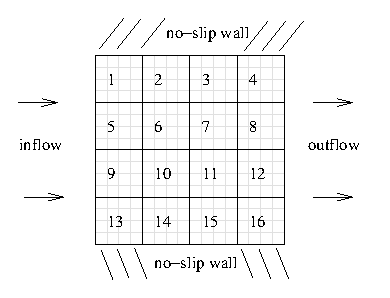
\includegraphics[width=4in]{./F_AdvancedTopics/bc_example1}
\caption{\label{fig:bc_example1}Two-dimensional example with 16 - 4$^2$grids with
{\tt INLET}, {\tt OUTLET}, and {\tt NO\_SLIP\_WALL} boundary conditions.
The numbers refer to the grid number.}
\end{figure}
%%%%%%%%%%%%%%%%%%%%%%%%%%%%%%%%%%%%%

\item Figure \ref{fig:bc_example2} demonstrates a problem with periodicity in the x-direction.
In this case, the low-x boundary condition for grid 1 is {\tt PERIODIC}.  Note there are some
similarities between {\tt PERIODIC} and {\tt INTERIOR} boundary conditions when
it comes to filling ghost cells in that ghost cell values are simply copied in from the valid
region of another grid.  In fact, one can think of {\tt PERIODIC} as just
a special type of {\tt INTERIOR} boundary condition.
For the other boundary conditions types, the user can write custom boundary 
conditions routines to fill ghost cells, which can involve setting ghost cell values 
directly, or using interior points and/or physical boundary conditions in some stencil operation.
%%%%%%%%%%%%%%%%%%%%%%%%%%%%%%%%%%%%%
\begin{figure}[tb]
\centering
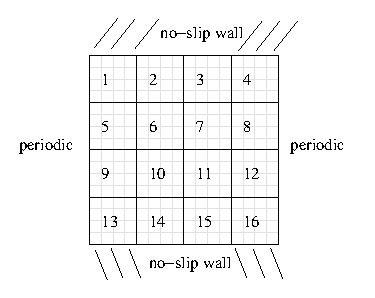
\includegraphics[width=4in]{./F_AdvancedTopics/bc_example2}
\caption{\label{fig:bc_example2}Two-dimensional example with 16 - 4$^2$grids with
{\tt PERIODIC} and {\tt NO\_SLIP\_WALL} boundary conditions.
The numbers refer to the grid number.}
\end{figure}
%%%%%%%%%%%%%%%%%%%%%%%%%%%%%%%%%%%%%

\item Now, consider an example with refined grids.  Figure \ref{fig:bc_example3}
contains three grids at the next level of refinement.  In this case, for grid 1,
all of the boundary condition types are {\tt INTERIOR}, even though the neighboring
valid region data is at a coarser level of refinement.  For grid 2, the low-y
boundary condition is {\tt NO\_SLIP\_WALL}, and the other three walls are {\tt INTERIOR}.
%%%%%%%%%%%%%%%%%%%%%%%%%%%%%%%%%%%%%
\begin{figure}[tb]
\centering
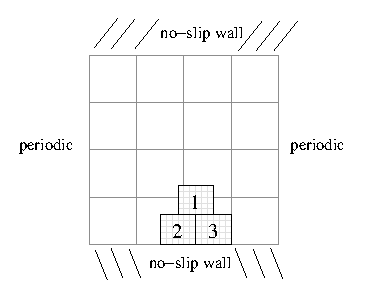
\includegraphics[width=4in]{./F_AdvancedTopics/bc_example3}
\caption{\label{fig:bc_example3}Two-dimensional example with 3 grids at a finer
resolution than the base grid.}
\end{figure}
%%%%%%%%%%%%%%%%%%%%%%%%%%%%%%%%%%%%%
\end{itemize}
\cleardoublepage

\subsection{Implementation}
Typically, we read in integer values from the inputs file for {\tt bc\_x\_lo}, 
{\tt bc\_x\_hi}, {\tt bc\_y\_lo}, etc., that correspond to the physical boundary condition types.
We then build a {\tt bc\_tower} object which is an array of {\tt bc\_level} objects, one for
each level of refinement.  The {\tt bc\_level} contains several integer array data structures,
as can be seen in {\tt BoxLib/Src/F\_BaseLib/define\_bc\_tower.f90}:
\begin{lstlisting}[backgroundcolor=\color{light-green}]
type bc_level

   ! 1st index is the grid number (grid "0" corresponds to the prob domain)
   ! 2nd index is the direction (1=x, 2=y, 3=z)
   ! 3rd index is the side (1=lo, 2=hi)
   ! 4th index is the variable (only assuming 1 variable here)
   integer, pointer :: phys_bc_level_array(:,:,:) => Null()
   integer, pointer ::  adv_bc_level_array(:,:,:,:) => Null()
   integer, pointer ::  ell_bc_level_array(:,:,:,:) => Null()

end type bc_level
\end{lstlisting}
Each level has a {\tt phys\_bc\_level\_array(0:ngrids,dim,2)} array, where {\tt ngrids} is the number of
grids on that level, {\tt dim} is the dimensionality of the simulation, and the third index refers to
the lower or upper edge of the grid in that coordinate direction.  This stores the {\it physical description}
of the boundary type ({\tt INLET}, {\tt OUTLET}, etc.), which is independen of the variables that live on
the grid.  The {\tt phys\_bc\_level\_array(0,:,:)} refers to the entire domain.  If an edge of a grid is not
a physical boundary, then it is set to a default value, typically {\tt INTERIOR}.  These boundary condition
types are used to interpret the actual method to fill the ghost cells for each variable, as described
in {\tt adv\_bc\_level\_array} and {\tt ell\_bc\_level\_array}.

Whereas {\tt phys\_bc\_level\_array} provides a physical description of the type of boundary, the array
{\tt adv\_bc\_level\_array} describes the action taken (e.g. reflect, extrapolate, etc.) for each 
variable when filling physical ghost cells on domain boundaries.  The prefix ``{\tt adv\_}'' is somewhat
of a misnomer, as this data structure was originally intended to tell advection (or hyperbolic) solvers
how to fill ghost cells, but now are generally used to fill physical domain boundary ghost cells in any
instance where the user needs to set them.
The form of this array is {\tt adv\_bc\_level\_array(0:ngrids,dim,2,nvar)}
where the additional component, nvar, allows for different state variable that lives on a grid to have 
different boundary condition actions associated with it.  For example, you could have {\tt nvar=1}
correspond to the x-velocity, {\tt nvar=2} correspond to density, and {\tt nvar=3} correspond to pressure.
In the {\tt BoxLib/Tutorials/HeatEquation\_EX2\_F/} tutorial, there is only one variable, $\phi$, so
obviously {\tt nvar=1} shall correspond to $\phi$.  When we build the {\tt adv\_bc\_level\_array},
we first set all values to {\tt INTERIOR}, and then overwrite any physical domain boundary condition types,
as given in {\tt phys\_bc\_level\_array}.  The {\tt adv\_bc\_level\_array} types supported by default are
(as listed in {\tt BoxLib/Src/F\_BaseLib/bc.f90}):
\begin{lstlisting}[backgroundcolor=\color{light-green}]
integer, parameter, public :: INTERIOR     =  0

integer, parameter, public :: REFLECT_ODD  =  20
integer, parameter, public :: REFLECT_EVEN =  21
integer, parameter, public :: FOEXTRAP     =  22
integer, parameter, public :: EXT_DIR      =  23
integer, parameter, public :: HOEXTRAP     =  24
\end{lstlisting}

To manually fill ghost cells, we call {\tt multifab\_physbc}, passing in the state multifab
along with the {\tt adv\_bc\_level\_array}.  The subroutines {\tt physbc\_1d/2d/3d} in
{\tt BoxLib/Src/F\_BaseLib/multifab\_physbc.f90}, indicate how to fill ghost cells.  For example,
\begin{lstlisting}[backgroundcolor=\color{light-green}]
subroutine multifab_physbc(s,start_scomp,start_bccomp,ncomp,the_bc_level)

  integer        , intent(in   ) :: start_scomp,start_bccomp,ncomp
  type(multifab) , intent(inout) :: s
  type(bc_level) , intent(in   ) :: the_bc_level

  ! Local
  integer                  :: lo(get_dim(s)), hi(get_dim(s))
  integer                  :: i,ng,dm
  integer                  :: scomp,bccomp
  real(kind=dp_t), pointer :: sp(:,:,:,:)
    
  ng = nghost(s)
  dm = get_dim(s)
    
  do i=1,nboxes(s)
     if ( multifab_remote(s,i) ) cycle
     sp => dataptr(s,i)
     lo = lwb(get_box(s,i))
     hi = upb(get_box(s,i))
     select case (dm)
     case (2)
        do scomp=start_scomp,start_scomp+ncomp-1
           bccomp = start_bccomp + scomp - start_scomp
           call physbc_2d(sp(:,:,1,scomp), lo, hi, ng, &
                          the_bc_level%adv_bc_level_array(i,:,:,bccomp))
        end do
...

subroutine physbc_2d(s,lo,hi,ng,bc)

  use bl_constants_module
  use bc_module

  integer        , intent(in   ) :: lo(:),hi(:),ng
  real(kind=dp_t), intent(inout) :: s(lo(1)-ng:,lo(2)-ng:)
  integer        , intent(in   ) :: bc(:,:)

  ! Local variables
  integer :: i,j

  !!!!!!!!!!!!!
  ! LO-X SIDE
  !!!!!!!!!!!!!

  if (bc(1,1) .eq. EXT_DIR) then
     ! set all ghost cell values to a prescribed dirichlet
     ! value; in this example, we have chosen 1
     do j = lo(2)-ng, hi(2)+ng
        s(lo(1)-ng:lo(1)-1,j) = 1.d0
     end do
  else if (bc(1,1) .eq. FOEXTRAP) then
     ! set all ghost cell values to first interior value
     do j = lo(2)-ng, hi(2)+ng
        s(lo(1)-ng:lo(1)-1,j) = s(lo(1),j)
     end do
...
\end{lstlisting}

{\tt ell\_bc\_level\_array} is the analog to {\tt adv\_bc\_level\_array} for the linear solvers in
\BoxLib.  These will be described in Section \ref{Sec:Linear Solvers}.

\section{Multiple Levels of Refinement}\label{Sec:Refinement}
In the {\tt BoxLib/Tutorials/HeatEquation\_EX3\_F/} tutorial, we have expanded our example
to the cases of multiple levels of refinement, with the grids fixed in space.  Note that there is
currently no subcycling support for Fortran90 \BoxLib, so in this example we advance all the grids
with the same time step, and perform synchronization operations between levels.\\

The big change for this tutorial is that we use a "multilevel layout" {\tt ml\_layout} 
rather than a {\tt layout}, and also {\tt multifab phi} and {\tt dx} are now {\tt nlevs} sized arrays.
After initializing or updating $\phi$, we must fill all ghost cell and synchronize the solution between
levels.  After we make the fluxes, we must synchronize the fluxes to maintain conservation.\\

There are three key subroutines for filling ghost cells and synchronizing data in multilevel applications.
Each of these involves a coarse level and a fine level:
\begin{itemize}

\item {\tt ml\_cc\_restriction} sets coarse cell-centered values equal to the average of the fine
  cells covering it.

\item {\tt ml\_edge\_restriction} sets coarse edge-centered values (such as fluxes) equal to the average
  of the fine edges covering it.

\item {\tt multifab\_fill\_ghost\_cells} fills fine ghost cells using interpolation from the underlying coarse
  data.  Note that this operation does not affect ghost cells that would be filled by {\tt multifab\_fill\_boundary}
  or {\tt multifab\_physbc}.

\end{itemize}

\section{Adaptive Mesh Refinement}\label{Sec:AMR}
Now fully implemented in {\tt BoxLib/Tutorials/HeatEquation\_EX4\_F/}.  The basic idea is
to ``tag'' the cells you with to refine in {\tt BoxLib/Src/F\_BaseLim\b/tag\_boxes.f90}.  To write
your own customized tagging criteria, copy {\tt tag\_boxes.f90} into your local directory and modify
it, since this copy will take precedence over the version in the \BoxLib~source.

There are several new
parameters that can be set via an inputs file:
\begin{itemize}
\item {\tt amr\_buf\_width}: radius (in cells) of tagged cells in addition to those already tagged due to the criteria in {\tt tag\_boxes.f90}.
\item {\tt cluster\_minwidth}: any newly created grids must be at least this many cells in each direction.
\item {\tt cluster\_blocking\_factor}: any newly created grids must have an integer multiple of this many cells in each direction.
\item {\tt cluster\_min\_eff}: This is a real number between 0 and 1 that controls how tightly the newly created grids match the tagged cells.  As this value approaches 1, you will have more, smaller grids.  Another way to think of this is that during the grid creation process, at least 100$\times${\tt cluster\_min\_eff} percent of the cells in each grid at which the grid creation occurs must be tagged cells.
\item {\tt regrid\_int}: frequency, in time steps, on when to regrid the simulation.
\end{itemize}
It is worth playing around with the inputs files to see what effect these parameters have on the grid structure.

\section{Linear Solvers}\label{Sec:Linear Solvers}
The tutorial code {\tt BoxLib/Tutorials/HeatEquation\_EX5\_F/} contains an implicit version of the heat equation 
example.  Fortran90 \BoxLib contains a ``cell-centered'' multigrid solver that solves linear systems of the form:
\begin{equation}
(\alpha\mathcal{I} - \nabla\cdot\beta\nabla)\phi = \text{RHS},
\end{equation}
where $\alpha, \phi$, and RHS are cell-centered \MultiFab~s, and $\beta$ is an array of \MultiFab~s that 
are nodal in exactly one direction (i.e., one face-centered \MultiFab for each spatial direction).
The Laplacian-like term in the left-hand-side can be discretized in several ways.  The simplest discretization
option is similar to a 5-point (7-point in 3D) Laplacian:
\begin{eqnarray}
\nabla\cdot\beta\nabla\phi_{ij} &=&
\frac{1}{\Delta x} \left[\beta_{i+\myhalf,j}\frac{\phi_{i+1,j} - \phi_{ij}}{\Delta x} - \beta_{i-\myhalf,j}\frac{\phi_{ij} - \phi_{i-1,j}}{\Delta x}\right]\nonumber\\
&&+ \frac{1}{\Delta y} \left[\beta_{i,j+\myhalf}\frac{\phi_{i,j+1} - \phi_{ij}}{\Delta y} - \beta_{i,j-\myhalf}\frac{\phi_{ij} - \phi_{i,j-1}}{\Delta y}\right].
\end{eqnarray}
A fully implicit discretization of the heat equation,
\begin{equation}
\frac{\phi^{n+1} - \phi^n}{\Delta t} = \left[\nabla\cdot(\nabla\phi)\right]^{n+1},
\end{equation}
is equivalent to
\begin{equation}
(\mathcal{I} - \Delta t\nabla\cdot\nabla)\phi^{n+1} = \phi^n.
\end{equation}
Thus, we will set $\alpha=1$, each $\beta=\Delta t$, and RHS = $\phi^n$.
